\documentclass{article}

\title{Practice-1}
\author{2347139}
\date{\today}


\usepackage{listings}
\usepackage{color}
\usepackage{graphicx}

\definecolor{dkgreen}{rgb}{0,0.6,0}
\definecolor{gray}{rgb}{0.5,0.5,0.5}
\definecolor{mauve}{rgb}{0.58,0,0.82}

\lstset{frame=tb,
  language=Java,
  aboveskip=3mm,
  belowskip=3mm,
  showstringspaces=false,
  columns=flexible,
  basicstyle={\small\ttfamily},
  numbers=left,
  numberstyle=\tiny\color{gray},
  keywordstyle=\color{blue},
  commentstyle=\color{dkgreen},
  stringstyle=\color{mauve},
  breaklines=true,
  breakatwhitespace=true,
  tabsize=3
}
\begin{document}
\maketitle
\begin{lstlisting}
    // P-1 Create Java program by using Minimum 5 Variables, one General Method, Default Constructor, Parameterized Constructor, Different Parameterized constructor(Constructor Overloading)

class Builder {
    public String botName;
    protected String discordToken;

    Builder(String botName, String discordToken) { // paramerterized constructor
        if (discordToken.isEmpty()) {
            System.out.println("Token not found");
        }
        this.botName = botName;
        this.discordToken = discordToken;
    }

    public void showBotDetails() {
        System.out.println("Discord Bot with " + botName + " created in your account");

    }

    public void createGuild(String guildName) {
        System.out.println("Created a guild " + guildName + " associated to the bot");
    }

    public void getBotPermission(int permission) {
        boolean isAdmin = true;
        boolean isMod = true;
        boolean BAN_MEMBERS = true;
        boolean KICK_MEMBERS = true;
        if (permission == 0) {
            System.out.println("The Bot created has 0 permission");
        }
        if (isAdmin && isMod && BAN_MEMBERS && KICK_MEMBERS) {
            System.out.println("The Bot is set full permission");
        }

    }

    public void showBotDetails(String clientName) {
        System.out.println("Discord Bot with " + botName + " created for client" + clientName);
    }

}

class SlashCommands extends Builder {

    SlashCommands() { // default constructor
        super("botName", "discordToken");
    }

    public void getMembers() { // method
        System.out.println("Getting members of the text channel");
        System.out.println("Channel members are : Elumeveguy\n" + //
                "Emojorekes\n" + //
                "Eroxihisom\n" + //
                "Ulelabutuk\n" + //
                "Ayibiciqeb\n" + //
                "Oguyocuxas\n" + //
                "Uxibabujen\n" + //
                "Epiwimaguk\n" + //
                "Idenefibiy\n" + //
                "Amarebamat");

    }

    public void slashCommand(String user) {
        // String command='ban';
        System.out.println("Ban User ");
        System.out.println("user " + user + " is banned");

    }

}

class Client extends SlashCommands {
    public String name;
    public String discordServer;

    Client(String name, String discordServer) {
        this.name = name;
        this.discordServer = discordServer;
    }

    Client(String discordServer) { // constructor overloading
        this.discordServer = discordServer;
    }

    public void getBotDetails() {
        if (name == null) {
            System.out.println("your Discord server name is : " + discordServer);
            return;
        }
        System.out.println("your account name is " + name);

    }
}

class Main {
    public static void main(String[] args) {
        Builder build = new Builder("arch-bot", "asak9889898ana");
        build.showBotDetails();
        build.createGuild("Moniter user actions");
        build.getBotPermission(0);
        SlashCommands cl = new SlashCommands();
        cl.getMembers();

        // client
        Client client = new Client("doe's server");
        build.showBotDetails("john");
        client.getBotDetails();

    }
}
\end{lstlisting}

\section*{Output}
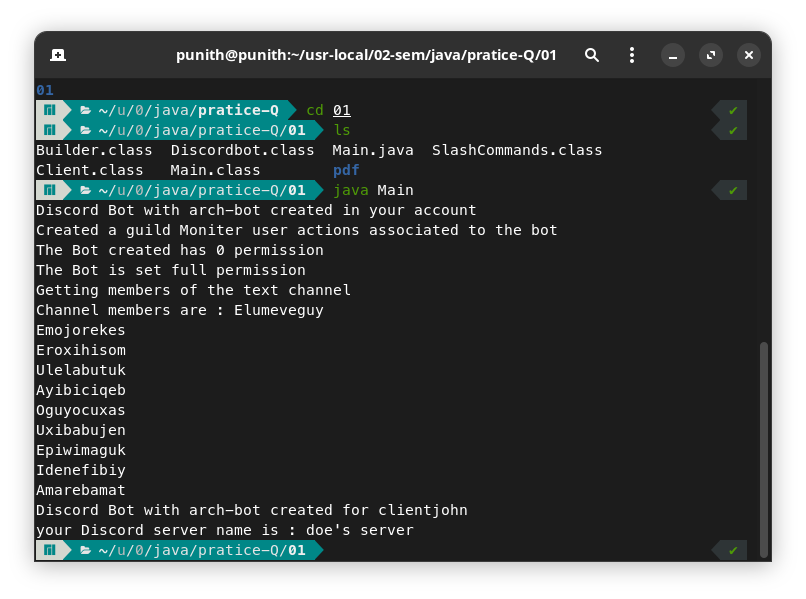
\includegraphics[width=11cm, height=9cm]{./images/01.png}

\end{document}
